\section{带电粒子和电磁场的相互作用}
对应电动力学课本第四章,占分10分左右。

\begin{question}
    当s'系相对s系的运动速度是任意方向时,四维时空的变换公式为:
    $$\mathbf{r}'=\mathbf{r}-\mathbf{v}t+(\frac{1}{\sqrt{1-\beta^2}}-1)\frac{\mathbf{v}}{v^2}(\mathbf{v}\cdot \mathbf{r}-v^2t)$$
    $$t'=\frac{t-\frac{1}{c^2}\mathbf{v}\cdot\mathbf{r}}{\sqrt{1-\beta^2}}$$
    其中$\beta=v/c$ 
 用四维势矢量的洛仑兹变换来推出运动带电粒子李纳—维希势。
\end{question}

\begin{question}
    什么是切仑科夫辐射?产生辐射的条件是什么?
\end{question}

\begin{question}
    什么是轫致辐射和同步辐射?并写出轫致辐射的电磁场。
    
    已知运动带电粒子的电磁场
    $$\mathbf{E}=\frac{e}{4\pi\varepsilon_0 c^2(r-\mathbf{r}\cdot \mathbf{v}/c)^3 }\left \{ c^2(1-\frac{v^2}{c^2})(\mathbf{r}-\frac{r\mathbf{v}}{c})+\mathbf{r} \times\left [ (\mathbf{r}-\frac{\mathbf{r}v}{c})\times \dot{\mathbf{v}} \right ] \right \}$$
    $$\mathbf{B}=\frac{\mathbf{r}}{cr}\times \mathbf{E}$$
\end{question}

\begin{question}   
    什么是同步辐射?并推出同步辐射的辐射功率的角分布(取如图所示坐标)。
    
    已知运动带电粒子的辐射功率的角分布
    $$\frac{\mathrm{d} P(t')}{\mathrm{d} \Omega}=\frac{e^2}{16\pi^2 \varepsilon_0 c^3}\frac{\left \{ \frac{\mathbf{r}}{r}\times\left [ (\frac{\mathbf{r}}{r}-\frac{\mathbf{v}}{c})\times \dot{\mathbf{v}} \right ]  \right \}^2}{(1-\frac{1}{c}\frac{\mathbf{r}\cdot \mathbf{v}}{r})^5}$$
    \begin{figure}[ht]
        \centering
        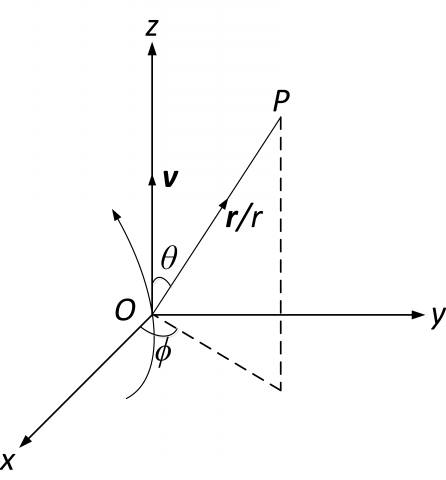
\includegraphics[height=3 cm]{images/q7_1.png}
        \caption{题\thequestion}
    \end{figure}
\end{question}

\begin{question}
    已知任意运动的带电粒子的电磁场为:
    $$\mathbf{E}=\frac{e}{4\pi\varepsilon_0 c^2(r-\mathbf{r}\cdot \mathbf{v}/c)^3 }\left \{ c^2(1-\frac{v^2}{c^2})(\mathbf{r}-\frac{r\mathbf{v}}{c})+\mathbf{r} \times\left [ (\mathbf{r}-\frac{\mathbf{r}v}{c})\times \dot{\mathbf{v}} \right ] \right \}$$
    $$\mathbf{B}=\frac{\mathbf{r}}{cr}\times \mathbf{E}$$
    1)求低速运动带电粒子的自有场。
    2)求低速运动带电粒子的辐射场。
    (按v/c展开,保留到v/c的一次项)
\end{question}

\begin{question}
    运动带电粒子辐射电磁波后,电磁波带走了能量,因此辐射场的反作用使带电粒子受到阻尼力,称为辐射阻尼力。在带电粒子作低速运动并且作周期运动的情况下,求对一个周期平均效应而言的辐射阻尼力。已知低速运动情况下粒子的辐射功率为 
    $$P(t')=\frac{e^2 \dot{\mathbf{v}}^2}{6\pi \varepsilon_0 c^3}$$
\end{question}